\section{The Frequency Bands}
	\begin{figure}[!ht]
	\centering
	\tikzset{every picture/.style={line width=0.75pt}} %set default line width to 0.75pt        
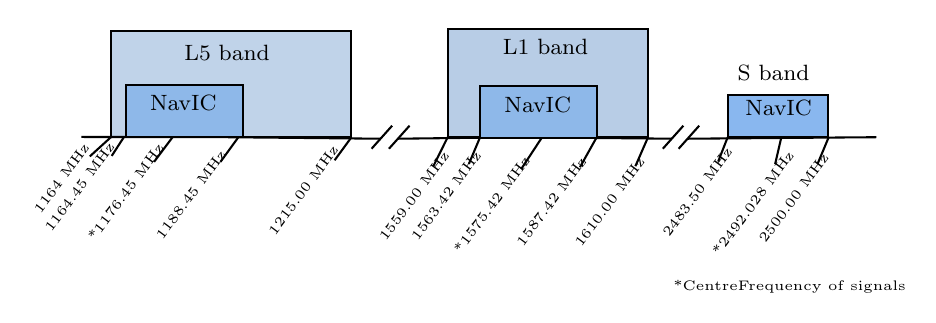
\begin{tikzpicture}[x=0.75pt,y=0.75pt,yscale=-1,xscale=1]
%uncomment if require: \path (0,471); %set diagram left start at 0, and has height of 471

%Shape: Rectangle [id:dp9517205987034671] 
\draw  [fill={rgb, 255:red, 192; green, 211; blue, 233 }  ,fill opacity=1 ] (92.53,176.6) -- (208.12,176.6) -- (208.12,227.79) -- (92.53,227.79) -- cycle ;
%Shape: Rectangle [id:dp3424557357689655] 
\draw  [fill={rgb, 255:red, 184; green, 205; blue, 230 }  ,fill opacity=1 ] (254.8,175.52) -- (351.33,175.52) -- (351.33,227.79) -- (254.8,227.79) -- cycle ;
%Shape: Rectangle [id:dp8560354037740456] 
\draw  [fill={rgb, 255:red, 137; green, 183; blue, 239 }  ,fill opacity=1 ] (389.7,207.67) -- (438,207.67) -- (438,227.79) -- (389.7,227.79) -- cycle ;
%Straight Lines [id:da4982550625943454] 
\draw    (78.33,227.67) -- (148.8,227.79) ;
%Straight Lines [id:da09038165069225701] 
\draw    (148.8,227.79) -- (222.43,228.52) ;
%Straight Lines [id:da6963693922945375] 
\draw    (230.82,228.52) -- (290.62,227.79) ;
%Straight Lines [id:da5101605840021868] 
\draw    (290.62,227.79) -- (362.75,228.52) ;
%Straight Lines [id:da4455724073590175] 
\draw    (218.13,233.34) -- (222.43,228.52) -- (228.04,222.24) ;
%Straight Lines [id:da44617587453109] 
\draw    (370.38,228.52) -- (461.33,227.79) ;
%Shape: Rectangle [id:dp9436860161134495] 
\draw  [fill={rgb, 255:red, 142; green, 184; blue, 233 }  ,fill opacity=1 ] (99.9,202.67) -- (156.33,202.67) -- (156.33,227.7) -- (99.9,227.7) -- cycle ;
%Straight Lines [id:da1306791733179924] 
\draw    (226.51,233.34) -- (230.82,228.52) -- (236.42,222.24) ;
%Straight Lines [id:da9755728827987384] 
\draw    (358.45,233.34) -- (362.75,228.52) -- (368.36,222.24) ;
%Straight Lines [id:da6153463426480046] 
\draw    (366.07,233.34) -- (370.38,228.52) -- (375.98,222.24) ;
%Straight Lines [id:da524212389543216] 
\draw    (92.53,227.79) -- (82.36,237.05) ;
%Straight Lines [id:da6359631954084011] 
\draw    (98.83,227.7) -- (92.93,236.8) ;
%Straight Lines [id:da4309637537474662] 
\draw    (122.33,227.67) -- (113.33,239.67) ;
%Straight Lines [id:da7084848716058743] 
\draw    (154.02,227.7) -- (145.34,239.67) ;
%Straight Lines [id:da9025278744467291] 
\draw    (208.45,227.79) -- (200.32,238.9) ;
%Straight Lines [id:da4288601859090342] 
\draw    (254.8,227.79) -- (247.94,241.67) ;
%Straight Lines [id:da6434353112428917] 
\draw    (270.26,228.16) -- (265,240.67) ;
%Straight Lines [id:da6934497348254585] 
\draw    (299.96,228.29) -- (290.19,243.19) ;
%Straight Lines [id:da08356280974055585] 
\draw    (326.33,228.29) -- (318.52,242.26) ;
%Straight Lines [id:da47170852835093413] 
\draw    (389.7,227.79) -- (385.12,239.51) ;
%Straight Lines [id:da39211419648473833] 
\draw    (415.47,228.16) -- (412.56,240.75) ;
%Straight Lines [id:da6629675504582904] 
\draw    (438.38,227.79) -- (433,240.67) ;
%Straight Lines [id:da16092426119270775] 
\draw    (351.33,227.79) -- (345.23,241.76) ;
%Shape: Rectangle [id:dp5224743842810824] 
\draw  [fill={rgb, 255:red, 142; green, 184; blue, 233 }  ,fill opacity=1 ] (270.26,203.12) -- (326.69,203.12) -- (326.69,228.16) -- (270.26,228.16) -- cycle ;

% Text Node
\draw (393.01,191.59) node [anchor=north west][inner sep=0.75pt]   [align=left] {{\footnotesize S band}};
% Text Node
\draw (396.7,208.67) node [anchor=north west][inner sep=0.75pt]   [align=left] {{\footnotesize NavIC}};
% Text Node
\draw (279.94,179.23) node [anchor=north west][inner sep=0.75pt]  [font=\footnotesize] [align=left] {L1 band};
% Text Node
%\draw (100.68,152.4) node [anchor=north west][inner sep=0.75pt]  [font=\scriptsize] [align=left] {ARNS / RNSS Band};
% Text Node
\draw (126.47,182.01) node [anchor=north west][inner sep=0.75pt]  [font=\footnotesize] [align=left] {L5 band};
% Text Node
\draw (109.89,206.05) node [anchor=north west][inner sep=0.75pt]   [align=left] {{\footnotesize NavIC}};
% Text Node
\draw (280.67,206.99) node [anchor=north west][inner sep=0.75pt]  [font=\normalsize] [align=left] {{\footnotesize NavIC}};
% Text Node
%\draw (252.7,152.4) node [anchor=north west][inner sep=0.75pt]  [font=\scriptsize] [align=left] {ARNS / RNSS Band};
% Text Node
%\draw (367.49,152.32) node [anchor=north west][inner sep=0.75pt]  [font=\scriptsize] [align=left] {RNSS/RDSS Band};
% Text Node
\draw (52.94,262.5) node [anchor=north west][inner sep=0.75pt]  [font=\scriptsize,rotate=-306.7] [align=left] {{\tiny 1164 MHz}};
% Text Node
\draw (58.07,271.48) node [anchor=north west][inner sep=0.75pt]  [font=\scriptsize,rotate=-306.7] [align=left] {{\tiny 1164.45 MHz}};
% Text Node
\draw (78.65,275.41) node [anchor=north west][inner sep=0.75pt]  [font=\scriptsize,rotate=-306.7] [align=left] {{\tiny *1176.45 MHz}};
% Text Node
\draw (111.71,275.12) node [anchor=north west][inner sep=0.75pt]  [font=\scriptsize,rotate=-306.7] [align=left] {{\tiny 1188.45 MHz}};
% Text Node
\draw (165.87,273.01) node [anchor=north west][inner sep=0.75pt]  [font=\scriptsize,rotate=-306.7] [align=left] {{\tiny 1215.00 MHz}};
% Text Node
\draw (219.28,275.78) node [anchor=north west][inner sep=0.75pt]  [font=\scriptsize,rotate=-306.7] [align=left] {{\tiny 1559.00 MHz}};
% Text Node
\draw (234.71,275.48) node [anchor=north west][inner sep=0.75pt]  [font=\scriptsize,rotate=-306.7] [align=left] {{\tiny 1563.42 MHz}};
% Text Node
\draw (255.1,281.42) node [anchor=north west][inner sep=0.75pt]  [font=\scriptsize,rotate=-306.7] [align=left] {{\tiny *1575.42 MHz}};
% Text Node
\draw (285.46,278.33) node [anchor=north west][inner sep=0.75pt]  [font=\scriptsize,rotate=-306.7] [align=left] {{\tiny 1587.42 MHz}};
% Text Node
\draw (313.45,278.62) node [anchor=north west][inner sep=0.75pt]  [font=\scriptsize,rotate=-306.7] [align=left] {{\tiny 1610.00 MHz}};
% Text Node
\draw (355.7,273.93) node [anchor=north west][inner sep=0.75pt]  [font=\scriptsize,rotate=-306.7] [align=left] {{\tiny 2483.50 MHz}};
% Text Node
\draw (379.59,282.47) node [anchor=north west][inner sep=0.75pt]  [font=\scriptsize,rotate=-306.7] [align=left] {{\tiny *2492.028 MHz}};
% Text Node
\draw (402.14,276.71) node [anchor=north west][inner sep=0.75pt]  [font=\scriptsize,rotate=-306.7] [align=left] {{\tiny 2500.00 MHz}};
% Text Node
\draw (362,295) node [anchor=north west][inner sep=0.75pt]  [font=\tiny] [align=left] {{\tiny *CentreFrequency of signals}};

\end{tikzpicture}

	\caption{Frequency bands of NavIC Signals}
	\label{figure:bandsfig}
	\end{figure}

\begin{table}[!ht]
	\small
	\centering
	%\subimport{table/}{table1.tex}
	\input{tables/bands}
	\caption{NavIC frequency bands}
	\label{table:bands}
	\end{table}

\noindent Satellite communication utilizes multiple frequency bands to accommodate different types of communication services and addresses various technical considerations. Here are some reasons why multiple frequency bands are used in satellite communication:
\\
\\
\textbf{Spectrum Allocation:} The electromagnetic spectrum is divided into various frequency bands to allocate different services and applications. This division ensures that different systems can operate without interfering with each other. By utilizing multiple frequency bands, satellite communication can effectively coexist with other wireless services and minimize interference issues.
\\
\\
\textbf{Signal Propagation Characteristics:} Different frequency bands exhibit unique propagation characteristics. Lower frequency bands, such as L band, have better signal penetration through obstacles and are less affected by atmospheric conditions, making them suitable for applications where signal reliability is crucial. Higher frequency bands, such as Ku band or Ka band, offer larger bandwidths and higher data transmission rates, making them ideal for applications requiring high-speed data transfer.
\\
\\
\textbf{Bandwidth and Capacity:} Different frequency bands offer varying bandwidths, and by utilizing multiple bands, satellite communication systems can increase overall capacity. This allows for the simultaneous transmission of multiple signals, accommodating a wide range of services such as television broadcasting, voice communication, internet access, and data transfer.
\\
\\
\textbf{Frequency Reuse and Interference Mitigation:} Satellite systems employ frequency reuse techniques to maximize the utilization of the available frequency spectrum. By using different frequency bands, satellite operators can reuse frequencies in different geographical areas without causing interference. This allows for efficient utilization of the limited spectrum resources.
\\
\\
\textbf{Regulation and International Coordination:} The allocation and usage of frequency bands are regulated by international bodies and national spectrum management organizations. These regulations help ensure efficient spectrum utilization, prevent interference between different systems, and promote global coordination and compatibility of satellite communication services.
\\
\\
In summary, the use of multiple frequency bands in satellite communication enables efficient spectrum utilization, accommodates different services, and addresses various technical considerations such as signal propagation, bandwidth, capacity, and interference mitigation. By leveraging the advantages offered by different frequency ranges, satellite systems can provide reliable, high-speed communication services to a wide range of applications and users.

\noindent The seven satellites in the NavIC constellation so far use two frequencies for providing positioning data — the L5 and S bands. This was because India hadn't received the International Telecommunication Union authorisation for using the L1 and L2 frequency bands, which are widely used worldwide for navigation services. The new satellites NVS-01 onwards, meant to replace these satellites, will also have L1 band. L1 is an interoperable frequency and can be used across all chipsets(of mobile devices), provided they use our signal architecture.

\subsection{L-band}
The L band offers several advantages for wireless communication systems, including a balance between signal propagation characteristics and antenna size. It provides good signal penetration through various atmospheric conditions, vegetation, and even some obstacles. These properties make it suitable for applications such as satellite communication, navigation systems, and mobile networks.

\noindent Satellite communication is one of the significant applications of the L band. Satellites in geostationary orbits often utilize this frequency range for broadcasting television signals, as well as for maritime, navigation and aeronautical communications. The L band allows for reliable and efficient transmission over long distances, making it a valuable resource for global connectivity. Because of satellites’ increased use, number and size, congestion has become a serious issue in the lower frequency bands.

\noindent L1 and L5 are specific frequencies within the L band that are used in Global Navigation Satellite Systems (GNSS), such as GPS (Global Positioning System), NavIC and Galileo. These frequencies play a crucial role in providing accurate positioning, navigation, and timing information.
\subsubsection{L1} 
L1 refers to the first frequency within the L band used by GNSS. In NavIC, the L1 frequency is centered around $1575.42$ MHz. The L1 signal carries the primary navigation message and is used for standard positioning and timing applications. It is widely used in various sectors, including transportation, surveying, and consumer applications like personal navigation devices and smartphones.
\subsubsection{L5}
L5, on the other hand, is an additional frequency introduced in modernized GNSS systems like GPS and Galileo. In NavIC, the L5 frequency is centered around $1176.45$ MHz. It was introduced to provide improved accuracy, integrity, and resistance to interference. The L5 signal carries more precise and reliable positioning information, making it particularly useful in critical applications that require high levels of accuracy, such as aviation, surveying, and scientific research.
The L1 frequency offers broad coverage and compatibility with legacy systems, while the L5 frequency provides more precise positioning and improved resistance to interference. The combination of these frequencies allows for more reliable and accurate navigation solutions, benefiting a wide range of industries and applications.
\subsection{S-band} 
The S band is another frequency range within the electromagnetic spectrum, located between the L band and the C band. It spans a frequency range of approximately $2$ to $4$ GHz. In NavIC, S band frequency is centred around $2492.028$ MHz. The S band finds applications in various fields, including communication, radar systems, satellite broadcasting, and scientific research.
\\
One of the primary uses of the S band is in satellite communication. Satellites in geostationary orbits often utilize S band frequencies for uplink and downlink communication with ground stations. The S band provides a good balance between antenna size and data capacity, making it suitable for broadcasting television signals, voice communication, and data transmission. However, the higher frequency bands typically give access to wider bandwidths, but are also more susceptible to signal degradation due to ‘rain fade’ (the absorption of radio signals by atmospheric rain, snow or ice).

\section{NavIC Architecture}	
The NavIC architecture is as shown in Fig \ref{figs:archfig}. It mainly consists of 
\begin{enumerate}
	\item Space segment 
	\item Ground segment 
	\item User segment 
\end{enumerate}

	\begin{figure}[!ht]
	\centering
	\includegraphics[width=\columnwidth]{figs/Architecture.jpg}
	\caption{NavIC Architecture}
	\label{figs:archfig}
	\end{figure}

\subsection{Space segment}
Space segment consists of a constellation of $7$ satellites. Three satellites of the constellation are placed in geostationary orbit, at $32.5^{\circ}$E, $83^{\circ}$E and $129.5^{\circ}$E respectively, and four satellites are placed in inclined geosynchronous orbit with equatorial crossing of $55^{\circ}$E and $111.75^{\circ}$E respectively, with inclination of $29^{\circ}$ (two satellites in each plane).

\subsection{Ground segment}
Ground segment takes care of operation and maintenance of the constellation. It consists of 
\begin{enumerate}
	\item ISRO Navigation Centre
	\item IRNSS Spacecraft Control Facility
	\item IRNSS Range and Integrity Monitoring Stations
	\item IRNSS Network Timing Centre
	\item IRNSS CDMA Ranging Stations
	\item Laser Ranging Stations
	\item Data Communication Network
\end{enumerate}

\subsection{User segment}
User segment consists of 
\begin{enumerate}
	\item A single frequency receiver having capability to receive SPS signal at either L1, L5 or S band frequency
	\item A multi-frequency receiver having capability to receive SPS signal at combination of L1, L5 and S band frequencies
	\item A multi-constellation receiver compatible with NavIC and other GNSS signals.
\end{enumerate}
\noindent The Figure\ref{figs:bandsfig} above specifies the radio frequency interface between space and user segments.

	\begin{figure}[!ht]
	\centering
	%\subimport{table/}{table1.tex}
	\tikzset{every picture/.style={line width=0.75pt}} %set default line width to 0.75pt        
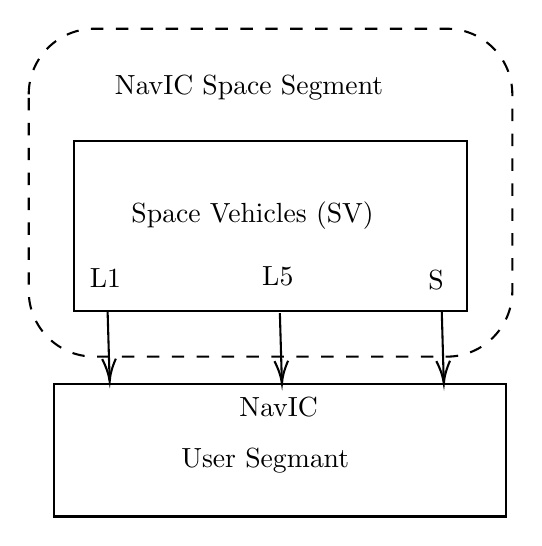
\begin{tikzpicture}[x=0.75pt,y=0.75pt,yscale=-1,xscale=1]
%uncomment if require: \path (0,406); %set diagram left start at 0, and has height of 406

%Shape: Rectangle [id:dp7411978076301706] 
\draw   (254,164) -- (443,164) -- (443,246) -- (254,246) -- cycle ;
%Straight Lines [id:da11098118487919195] 
\draw    (270,246) -- (270.94,278) ;
\draw [shift={(271,280)}, rotate = 268.32] [color={rgb, 255:red, 0; green, 0; blue, 0 }  ][line width=0.75]    (10.93,-3.29) .. controls (6.95,-1.4) and (3.31,-0.3) .. (0,0) .. controls (3.31,0.3) and (6.95,1.4) .. (10.93,3.29)   ;
%Shape: Rectangle [id:dp29610782491063636] 
\draw   (244,281) -- (462,281) -- (462,345) -- (244,345) -- cycle ;
%Straight Lines [id:da1330694648577655] 
\draw    (353,247) -- (353.94,279) ;
\draw [shift={(354,281)}, rotate = 268.32] [color={rgb, 255:red, 0; green, 0; blue, 0 }  ][line width=0.75]    (10.93,-3.29) .. controls (6.95,-1.4) and (3.31,-0.3) .. (0,0) .. controls (3.31,0.3) and (6.95,1.4) .. (10.93,3.29)   ;
%Straight Lines [id:da06268750746850027] 
\draw    (431,246) -- (431.94,279) ;
\draw [shift={(432,281)}, rotate = 268.36] [color={rgb, 255:red, 0; green, 0; blue, 0 }  ][line width=0.75]    (10.93,-3.29) .. controls (6.95,-1.4) and (3.31,-0.3) .. (0,0) .. controls (3.31,0.3) and (6.95,1.4) .. (10.93,3.29)   ;
%Rounded Rect [id:dp5981425610685245] 
\draw  [dash pattern={on 4.5pt off 4.5pt}] (232,141.6) .. controls (232,124.15) and (246.15,110) .. (263.6,110) -- (433.4,110) .. controls (450.85,110) and (465,124.15) .. (465,141.6) -- (465,236.4) .. controls (465,253.85) and (450.85,268) .. (433.4,268) -- (263.6,268) .. controls (246.15,268) and (232,253.85) .. (232,236.4) -- cycle ;

% Text Node
\draw (272,131) node [anchor=north west][inner sep=0.75pt]   [align=left] {NavIC Space Segment};
% Text Node
\draw (280,192) node [anchor=north west][inner sep=0.75pt]   [align=left] {Space Vehicles (SV)};
% Text Node
\draw (260,224) node [anchor=north west][inner sep=0.75pt]   [align=left] {L1};
% Text Node
\draw (343,223) node [anchor=north west][inner sep=0.75pt]   [align=left] {L5};
% Text Node
\draw (423,225) node [anchor=north west][inner sep=0.75pt]   [align=left] {S};
% Text Node
\draw (332,286) node [anchor=north west][inner sep=0.75pt]   [align=left] {NavIC};
% Text Node
\draw (304,311) node [anchor=north west][inner sep=0.75pt]   [align=left] {User Segmant};

\end{tikzpicture}

	\caption{the NavIC bands segment blocks}
	\label{figs:bandsfig}
	\end{figure}

\section{NavIC Services}
The NavIC provides basically two types of services:
	\begin{enumerate}
	\item Standard Positioning Service (SPS)
	\item Restricted Service (RS)
	\end{enumerate}
Both SPS and RS signals contain ranging codes that allow receivers to compute their travelling time from satellite to receiver, along with navigation data, in order to know the satellite’s position at any time. 
\subsection{Standard Positioning Service (SPS)}
	It is available to all civilian users free of charge and provides positioning, navigation, and timing information with a moderate level of accuracy. The SPS signals in NavIC primarily operate in the L5 and S frequency bands.
\subsection{Restricted Service (RS)}
The RS is intended for authorized users and offers enhanced accuracy, integrity, and availability compared to the SPS signals. The RS signals in NavIC operate in both the L5 and S bands and broadcast through a phased array antenna to keep required coverage and signal strength. 
\let\cleardoublepage\clearpage  %to remove blank page
%\end{document}
